\chapter{Présentation de l'entreprise}

\section{Valeo, un équipementier Automobile}

\subsection{Présentation de l'entreprise}

Valeo est un des leaders mondiaux dans l'activité d'équipementier automobile.

Depuis 1923, lors de création de la SAFF (\textit{Société Anonyme Française de Ferodo}) par Eugène Buisson, Valeo a toujours œuvré pour viser l'excellence. 

A partir de 1962 avec le rachat de la SOFICA (\textit{Société de Fabrication Industrielle de Chauffage et d'Aération}), l'entreprise s'ouvre vers l'Europe. C'est le début de multiples rachats et créations d'usines en europe (particulièrement en Espagne et en Italie).

C'est finalement en 1980 que le nom de Valeo (du latin : ``\textit{Je vais bien}") est adopté par le groupe.

Cette même année, Valeo inaugure son premier site aux États Unis, suivis en 1982 du Mexique.

L'année de mon stage, 2013, fut celle des 90 ans de Valeo, et toujours le même objectif :
\begin{quote}
\centering
\vspace{4mm}
	\textit{\textbf{``Accompagner les constructeurs et les automobilistes pour rendre les véhicules plus propres, performants et plus sûrs"}}\\
	\vspace{4mm}
	\textit{Jacques Aschenbroich - Communiqué des 90 ans de Valeo}
\end{quote}.

 \begin{figure}[H]
    \centering
    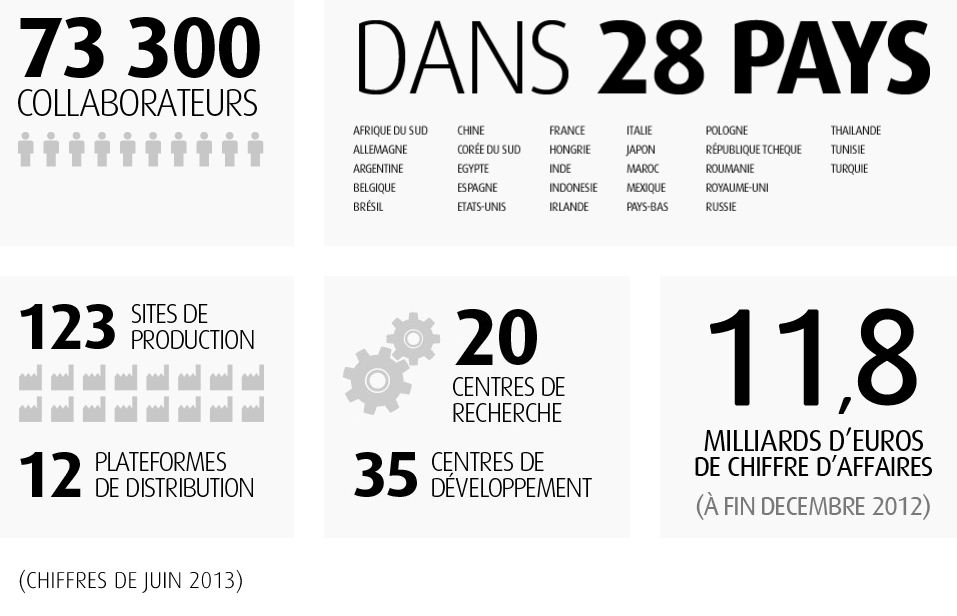
\includegraphics[height=6.6cm]{profil_valeo.jpg}
	\caption{Valeo aujourd'hui - Les chiffres clés - \cite{image.valeo.source} }\label{image.valeo} 
\end{figure}


\subsection{La structure interne de Valeo.}
Valeo est divisée en quatre ``Business Groups", à celà s'y ajoute un pole de deuxième monte : Valeo Service.

 \begin{figure}[H]
    \centering
    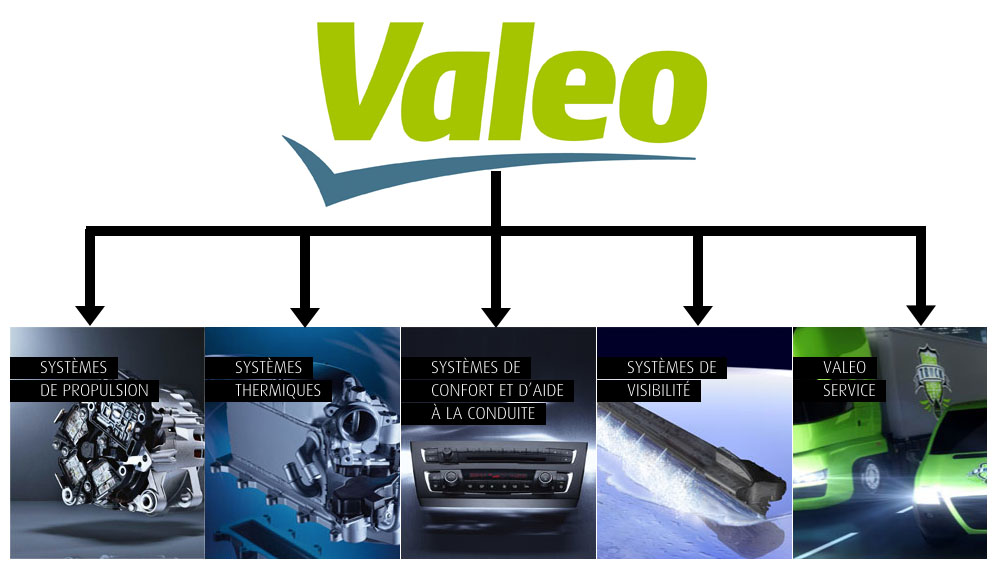
\includegraphics[height=7cm]{business_groups.jpg}
	\caption{4 Business Groups et Valeo Service - \cite{image.businessgroups.source} }\label{image.businessgroups} 
\end{figure}

\begin{quotation}
\begin{itshape}
Le Pôle Systèmes de Propulsion développe des solutions de propulsion innovantes visant à réduire la consommation de carburant et les émissions de CO2.\\
	\vspace{3mm}

Le Pôle Systèmes Thermiques développe et fabrique des systèmes, des modules et des composants assurant la gestion de l’énergie thermique du groupe motopropulseur ainsi que le confort de chaque passager dans l’habitacle.\\
	\vspace{3mm}

Le Pôle Systèmes de Confort et d’Aide à la Conduite développe des systèmes d’interface entre le conducteur, le véhicule et son environnement, contribuant à l’amélioration du confort et de la sécurité.\\
	\vspace{3mm}

Le Pôle Systèmes de Visibilité conçoit et produit des systèmes innovants qui assurent au conducteur une parfaite visibilité, contribuant ainsi à sa sécurité et à celle de ses passagers.\\
	\vspace{3mm}

Valeo Service fournit des pièces de rechange aux constructeurs automobile et au marché de la Rechange indépendante. Il propose à tous les réseaux de la rechange dans le monde une large gamme de produits et services.\\	
\end{itshape}\\
\textbf{Source : \url{http://www.valeo.com/nos-activites/}}

\end{quotation}

\subsection{La structure interne du Business Group : CDA}

J'ai effectué mon stage au sein du site d'Annemasse, site qui est rattaché au Business Group : Confort and Driving Assistance (CDA).\\
	\vspace{3mm}
	
 \begin{figure}[H]
    \centering
    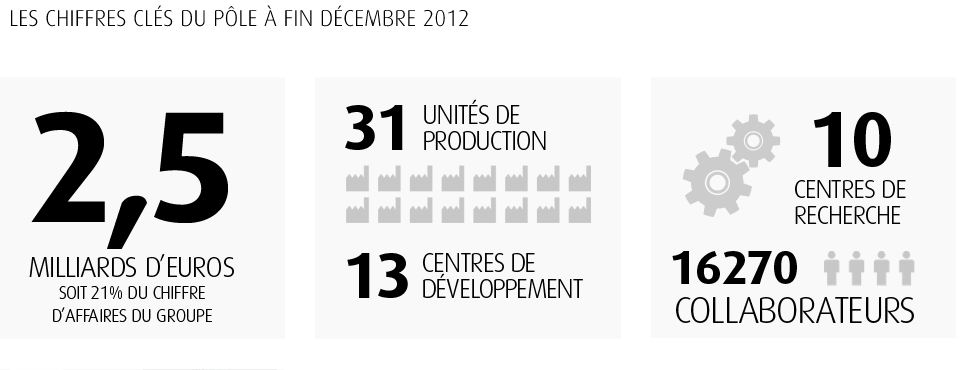
\includegraphics[height=5cm]{CDA.jpg}
	\caption{Les 4 Product Groups rattachés à CDA - \cite{image.cda.source} }\label{image.cda} 
\end{figure}

\begin{quotation}
\begin{itshape}
La mission du pôle systèmes de confort et d’aide à la conduite est de développer des systèmes d’interface entre le conducteur, le véhicule et son environnement tout en contribuant à l’amélioration du confort et de la sécurité.\\
	\vspace{3mm}
	
La conduite intuitive est le credo du pôle, grâce à quatre activités complémentaires~: \\
	\begin{itemize}
		\item Interaction ergonomique et simple du conducteur avec le véhicule
		\item Agilité de conduite par une meilleure perception de l’environnement
		\item Connectivité
		\item Accès personnalisé et sécurisé au véhicule
	\end{itemize}
\end{itshape}
\textbf{Source : \url{http://www.valeo.com/nos-activites/}}

\end{quotation}

\clearpage
\section{L'IS Shared Service Center - CDA France}

J'ai effectué mon stage au sein du \textbf{Centre Informatique de Service Partagé} (Information System Shared Service Center: IS SSC) du périmètre CDA France - Tunisie sous la tutelle de Marc LAURENT, le manager de cette section.\\

Valeo a structuré les ressources informatiques en structure que l'on appelle "\textbf{Cluster}".\\

Chaque Cluster informatique est en charge d'un certain nombre de sites, à la fois dans leur supervision, suivis de projets, que dans l'applicatif (ERP, Business Intelligence, Office Automation, DRP, Barcoding ...).

La partie infrastructure (réseau et serveur) ne fait pas partie des attributions de l'ISSS sauf en ce qui concerne l'ERP; cette partie est supervisée par un autre service et externalisée au maximum dans une optique de réduction des coûts.

Ainsi notre cluster se compose des sites suivants : 

	\begin{itemize}
		\item \textbf{Annemasse} (mon lieu de stage).
		\item \textbf{Nervers CIE}
		\item \textbf{Abbeville}
		\item \textbf{Mondeville}
		\item \textbf{Ben Arous} (\textit{Tunisie})
		\item \textbf{Créteil Europarc}
	\end{itemize}
	
	 \begin{figure}[H]
    	\centering
    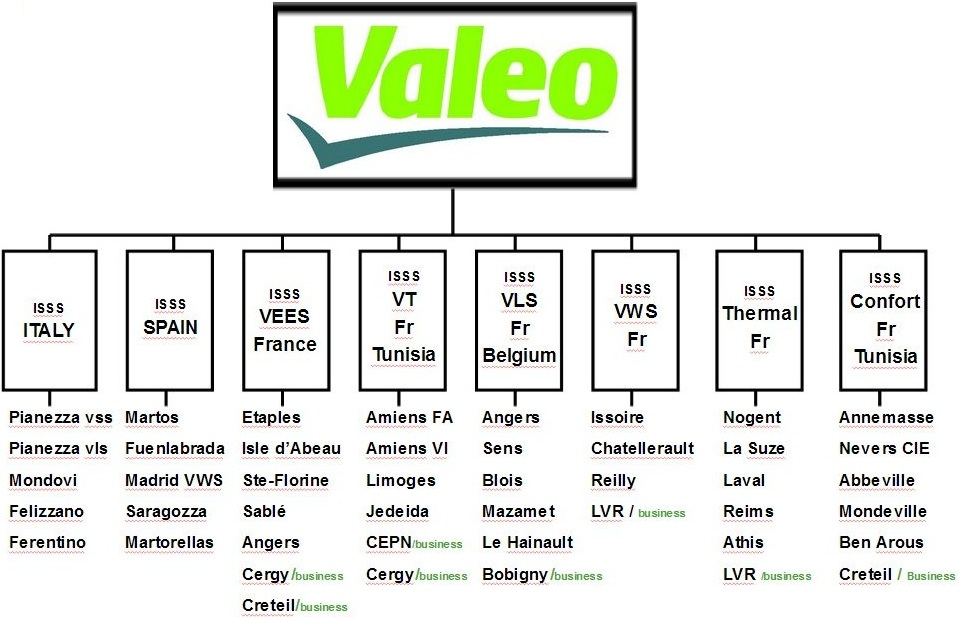
\includegraphics[height=8.3cm]{cluster.jpg}
	\caption{Les clusters informatiques - Europe de l'ouest}\label{image.cluster} 
\end{figure}

\clearpage
